% !Mode:: "TeX:UTF-8"
\documentclass{article}
\usepackage{graphicx}
\usepackage{CJK}

\usepackage{anysize}
\marginsize{2cm}{2cm}{-1cm}{2cm}

\begin{document}
\begin{CJK}{UTF8}{gkai} % gbsn: 宋体简化字;gkai 楷体简化字; bsmi 繁体宋书;bkai 繁体楷书
\makeatletter 
  \newcommand\figcaption{\def\@captype{figure}\caption} 
  \newcommand\tabcaption{\def\@captype{table}\caption} 
\makeatother
\renewcommand{\abstractname}{摘 \qquad 要}
\renewcommand{\contentsname}{\center 目\qquad\qquad录}
\renewcommand{\listfigurename}{图 \quad 示 \quad 目 \quad 录}
\renewcommand{\listtablename}{表 \quad 格 \quad 目 \quad 录}
\renewcommand{\appendixname}{附录}
\renewcommand{\refname}{\center 参 \quad 考 \quad 文 \quad 献}
%\renewcommand{\bibname}{专著}
\renewcommand{\indexname}{\center 索 \qquad 引}
\renewcommand{\figurename}{图}
\renewcommand{\tablename}{表}
%\renewcommand{\pagename}{页}

\title{图分析大作业文档}
\author{刘斌(2014013466) 李书昂(2014013431)}
\date{2015年12月30日}
\maketitle

\section{项目背景} % (fold)
	\paragraph{}
	图论在科技、社会上的应用日趋广泛,城市路网,社交网络,引文网络等众多类型的网络中都需要大量用到图论建模后使用相关理论去解决、优化相关问题。因此对图的分析并将分析结果可视化就显得尤为重要。
	\begin{figure}[htbp!]
		\begin{minipage}[t]{0.33\linewidth}
			\centering
			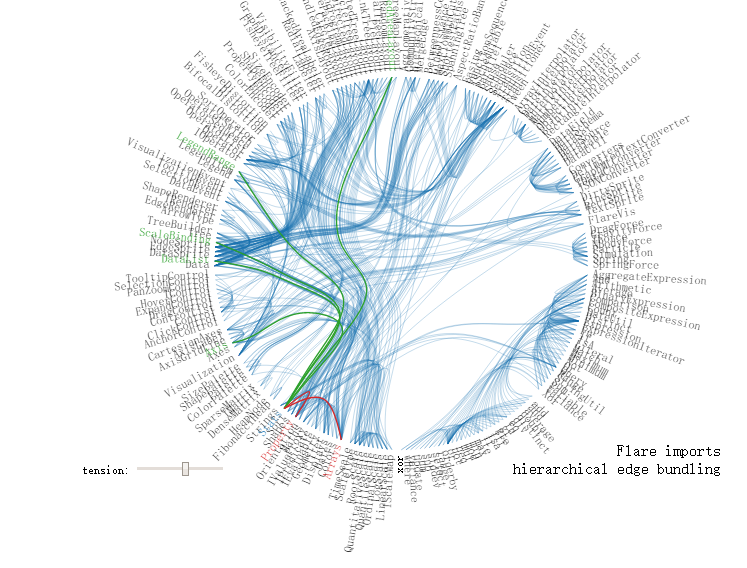
\includegraphics[width=2.2in]{graph.PNG}
			\caption{引文网络示例}
		\end{minipage}
		\begin{minipage}[t]{0.33\linewidth}
			\centering
			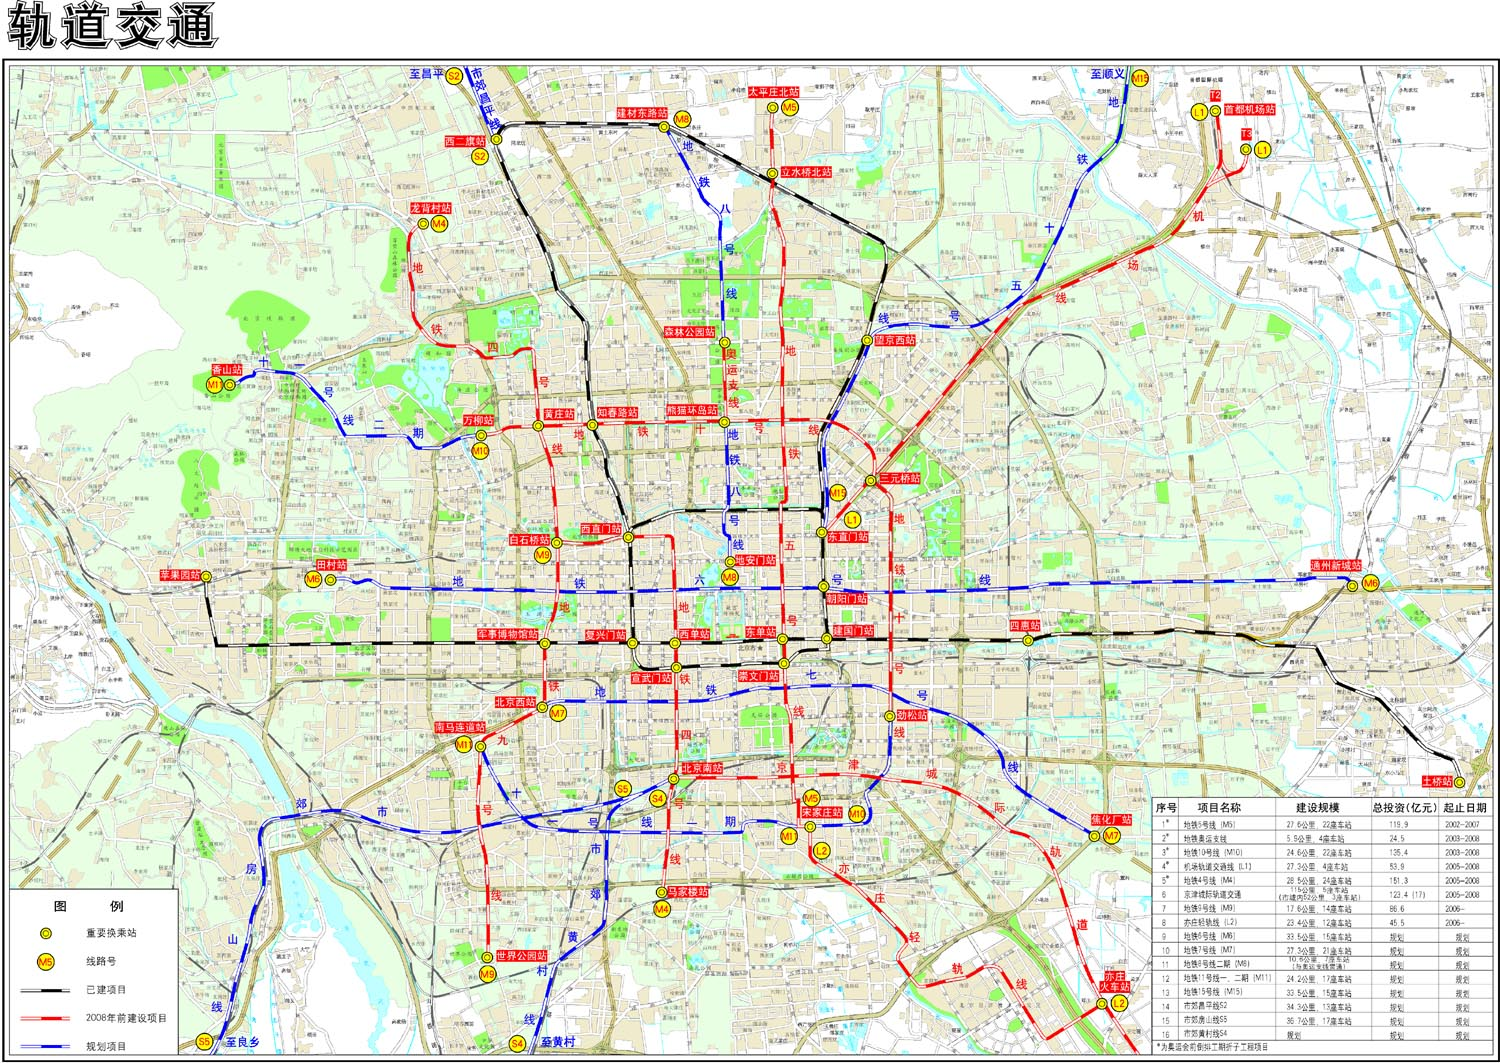
\includegraphics[width=2.2in]{graph_beijing_subway.jpg}
			\caption{城市路网示例}
		\end{minipage}
		\begin{minipage}[t]{0.33\linewidth}
			\centering
			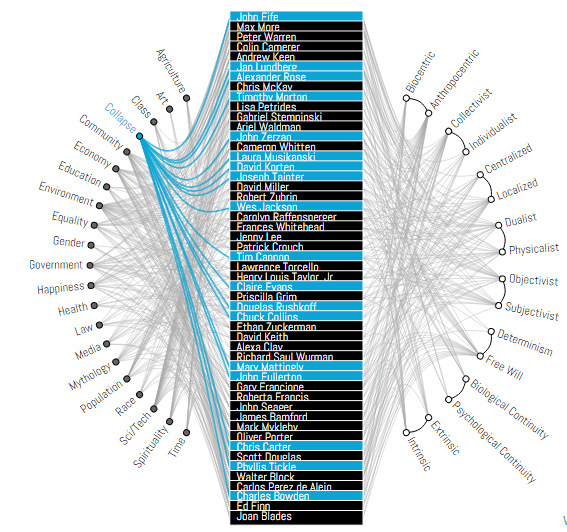
\includegraphics[width=2.2in]{graph_concept.PNG}
			\caption{概念图示例}
		\end{minipage}
	\end{figure}
% section 项目背景 (end)

\section{项目概况} % (fold)
	\paragraph{}
	我们完成了包括数据采集,网络图的构建,核心算法的实现,可视分析等所有必做功能和选做功能。其中数据采集自豆瓣,网络图使用json文件储存,核心算法使用JavaScript实现,可视分析使用Html + JS + CSS与用户进行交互。
% section 项目概况 (end)

\section{项目文件使用说明} % (fold)
	\paragraph{}
	首先运行服务器脚本server.bat(注意该脚本的位置应一直位于项目根目录下),然后在浏览器地址栏输入“$http://localhost:8000/$”即可进入主界面。在主界面内,可以对点进行拖动,可以单击选中某个点,此时右上角会显示出该点的详细信息。也可以鼠标悬停在某个点上,此时会显示出该点对应的电影名。
% section 项目文件使用说明 (end)

\section{数据采集} % (fold)
	\paragraph{}
	建立节点:访问豆瓣电影($http://movie.douban.com/$),选择豆瓣电影top250榜单,解析Html,获得当前页面的所有电影的详细信息,建立电影节点
	\paragraph{}
	建立边权:进入每一个电影的评论页面获取所有相关的用户评价。构建电影为节点网络(无向图),定义网络中边的含义,如果两个电影节点的评价中有一个相同用户,则边权+1,根据评分的相似程度确定遍全的小数部分(1/(abs(w1-w2)+1))。如果两个节点之间没有共同的用户,则视为这两个节点不联通。

% section 数据采集 (end)

\section{网络图的构建} % (fold)
	\paragraph{}
	由于采集下来的数据保存格式为txt,无法方便的读入网页,因此我们使用C++对txt文件进行处理,将其转化为json格式的文件。具体代码请查阅“data/changeDateToJSON/”目录下的changeDateToJSON工程。在网页中,节点被映射为圆,边被映射为直线,且直线的宽度为与边的权值相联系。此处我们使用的权值到宽度的函数是:
		$$width = Math.log(weight) / 2$$
% section 网络图的构建 (end)

\section{服务器搭建} % (fold)
	\paragraph{}
	由于网页中的数据需在打开网页时从本地加载,因此需要搭建一个简易的服务器以便传输文件。我们使用的是python2.7来搭键服务器,其源代码在源代码根目录下的server.bat中,该代码仅一行:python -m SimpleHTTPServer 8000。
	\\[\intextsep] 
	\begin{minipage}{\textwidth} 
	    \centering 
	    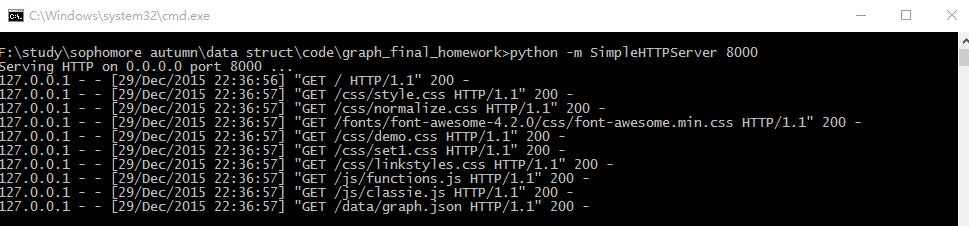
\includegraphics[width=0.9\linewidth]{server.PNG}
	    \figcaption{简易服务器效果图}
	\end{minipage} `'
	\\[\intextsep] 
% section 服务器搭建 (end)

\section{核心算法的实现} % (fold)
	\subsection{节点对的最短路径}
		\subsubsection{算法说明} % (fold)
			\paragraph{}
			由于此次项目中需要用到大量的最短路径,为了减轻后期计算压力,因此我们并未采用dijkstra算法来计算单源最短路径,而是在页面加载时便用warshall算法计算出所有节点对的最短路径和最短路径权值。在需要使用时直接查询即可。
		\subsubsection{操作说明}
			\paragraph{}
			在起点和终点框中输入起点和终点的index后点击确定即可得到最短路径的可视化表达。路径中涉及的点为红色,边为深黑色,未涉及的点颜色不变,边的不透明度变低。左下角将输出该路径的权值和。
		\\[\intextsep] 
		\begin{minipage}{\textwidth} 
		    \centering 
		    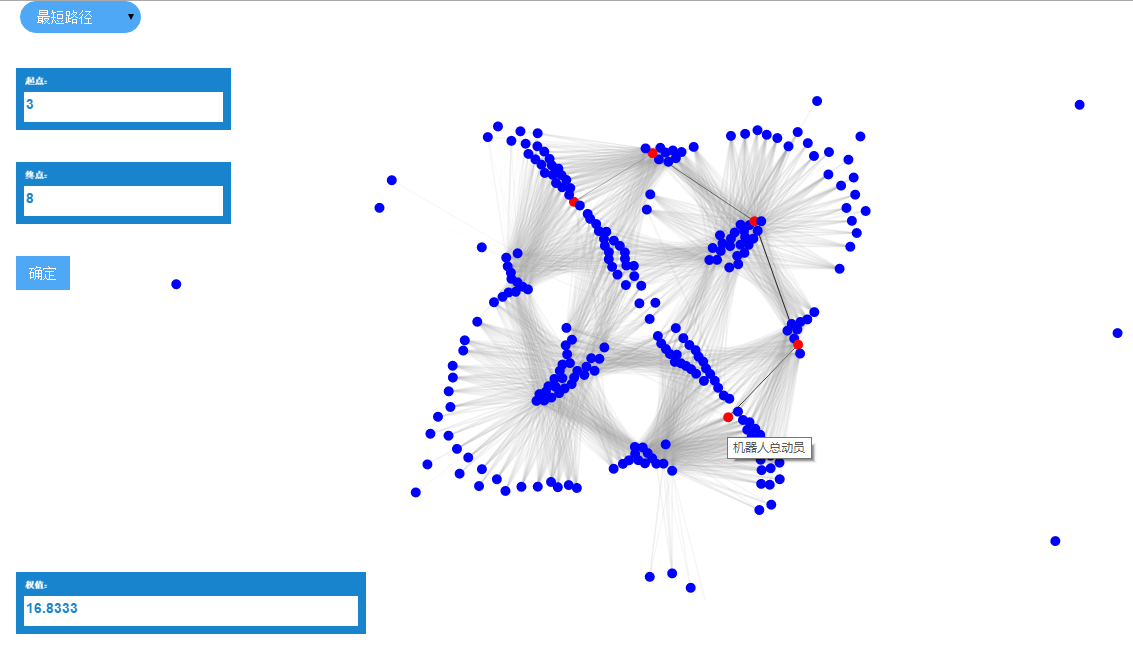
\includegraphics[width=0.9\linewidth]{path.PNG}
		    \figcaption{节点对的最短路径—效果预览}
		\end{minipage} 
		\\[\intextsep] 
		% subsubsection 算法说明 (end)

	\subsection{最小生成树}
		\subsubsection{最小生成树算法说明} % (fold)
			\paragraph{}
			最小生成树使用了prim算法来求解最小生成树。
		\subsubsection{操作说明}
			\paragraph{}
			输入根节点,调节最小权值限定,即可得到最小生成树的可视化表达。其中跟节点用黄色标注,其余属于该生成树的节点用红色标注,不属于该生成树的节点颜色不变。树中的边颜色为深黑色,不在树中的边不透明度变低。左下角将输出该生成树的权值和。
		\\[\intextsep] 
		\begin{minipage}{\textwidth} 
		    \centering 
		    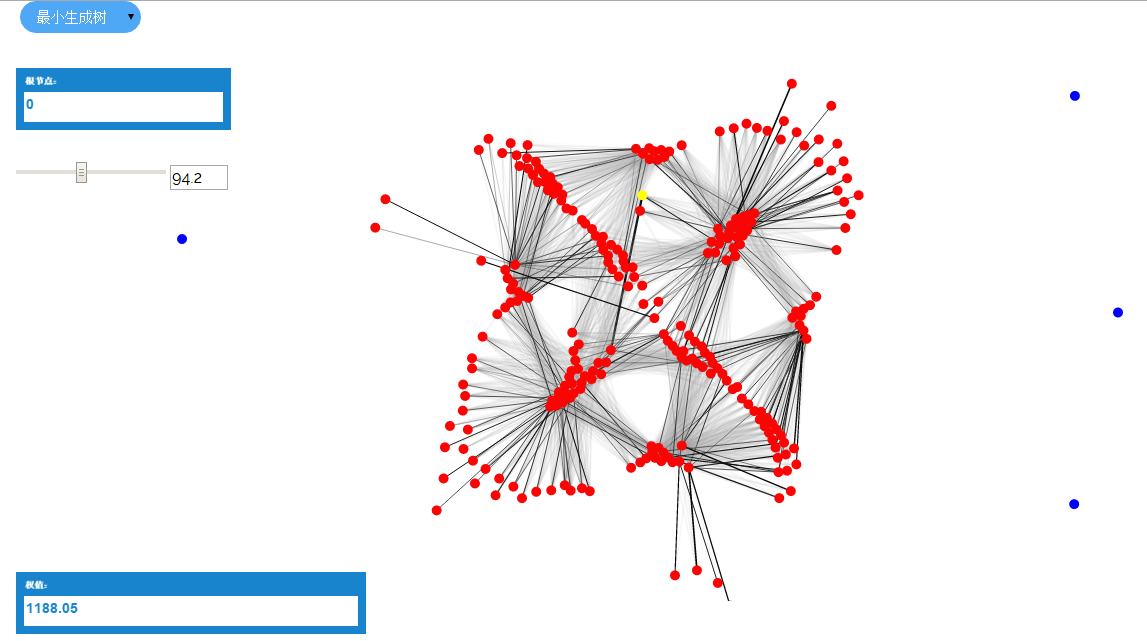
\includegraphics[width=0.9\linewidth]{mst.PNG}
		    \figcaption{最小生成树—效果预览}
		\end{minipage} 
		\\[\intextsep] 	
		% subsubsection 算法说明 (end)

	\subsection{中心度}
		\subsubsection{介数中心度算法说明} % (fold)
			\paragraph{}
			介数中心度使用warshall算法的结果,遍历所有节点对的最短路径即可获得所有节点对应的介数中心度。
		\subsubsection{操作说明} % (fold)
			\paragraph{}
			当选择中心度时,网页默认显示介数中心度。此外,点击介数中心度按钮即可得到介数中心度的可视化表达,颜色越接近红色度越高。
		\\[\intextsep] 
		\begin{minipage}{\textwidth} 
		    \centering 
		    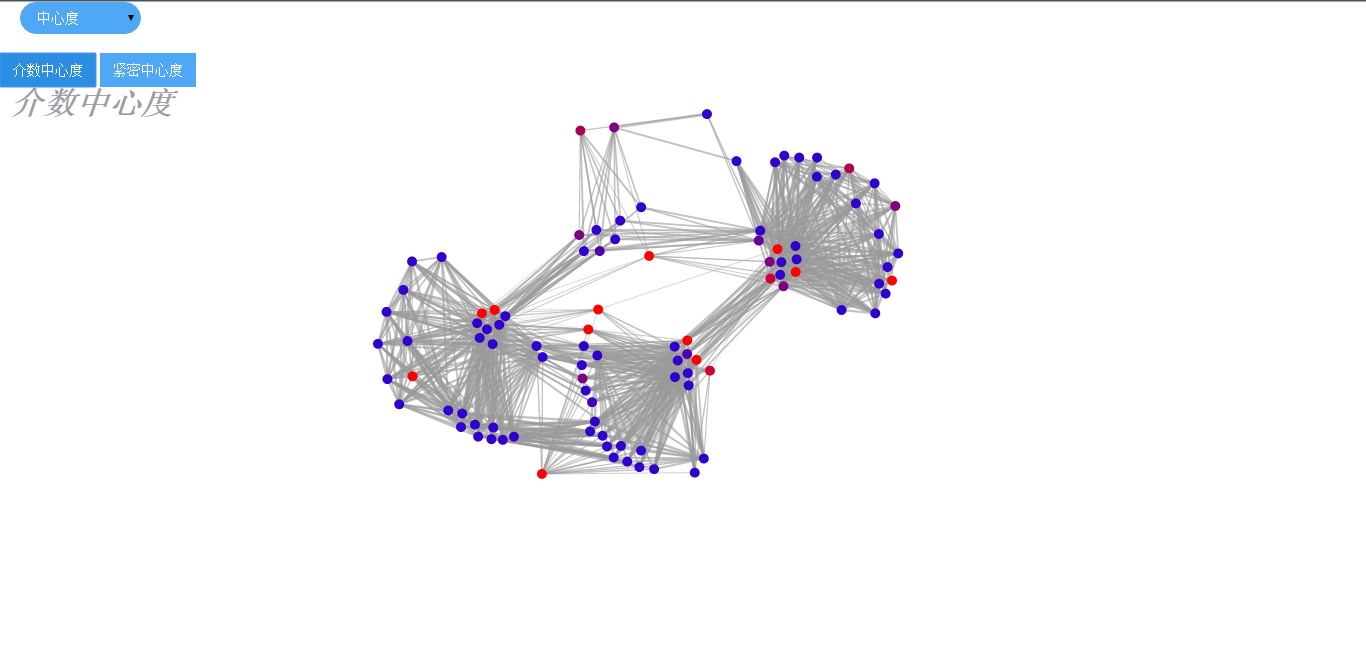
\includegraphics[width=0.9\linewidth]{bc.PNG}
		    \figcaption{介数中心度—效果预览}
		\end{minipage} 
		\\[\intextsep] 

		\subsubsection{紧密中心度算法说明}
			\paragraph{}
			介数中心度使用warshall算法的结果,遍历所有节点对的最短路径即可获得所有节点对应的介数中心度,颜色越接近红色度越高。
		\subsubsection{操作说明} % (fold)
			\paragraph{}
			点击紧密中心度按钮即可得到紧密中心度的可视化表达。		
		\\[\intextsep] 
		\begin{minipage}{\textwidth} 
		    \centering 
		    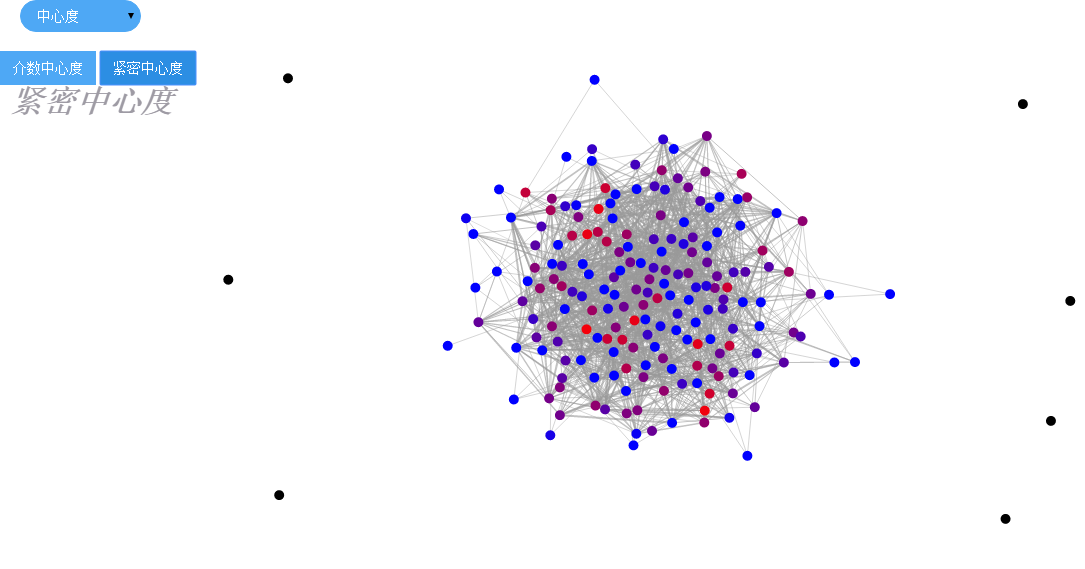
\includegraphics[width=0.9\linewidth]{cc.PNG}
		    \figcaption{紧密中心度—效果预览}
		\end{minipage} 
		\\[\intextsep] 
		% subsubsection 算法说明 (end)

	\subsection{连通分量}
		\subsubsection{连通分量算法说明} % (fold)
			\paragraph{}
			连通分量中使用了深度优先搜索算法对所有节点进行了一遍遍历,并在遍历过程中对每一个节点赋予特定的颜色值(将与当前节点连通的节点颜色设置为当前节点的颜色,若无节点与当前节点连通,则重新寻找一个搜索起点,并重新设置一个颜色值。)同时为了处理“阈值较小时边很多会遮盖节点,影响节点的显示,阈值较大时边很少,不容易从图中看出”的矛盾,需要在网页中我们根据将要展示的边的条数来调整边的不透明度。我们采用的函数是
			 $$opacity = 1 / (1 + Math.log(link\_count + 1))$$
			\paragraph{}
			 其中$opacity$为边的不透明度,$link\_count$为将展示的边的数量,大致范围为0到1200。经过该函数的映射,边的不透明度的范围约是0.1到1,且边的数量越少,不透明度越高,能达到较好的展示效果。
		\subsubsection{操作说明} % (fold)
			\paragraph{}
			拖动滑动条改变最小阈值t或直接在输入框中输入阈值t即可得到阈值为t时的连通分量可视化表达。其中相同连通分量的颜色相同,不同连通分量的颜色一般不同(不过当连通分量的数目大于20时便会重复)。同一个连通分量内的边与两端顶点的颜色相同。
		\\[\intextsep] 
		\begin{minipage}{\textwidth} 
		    \centering 
		    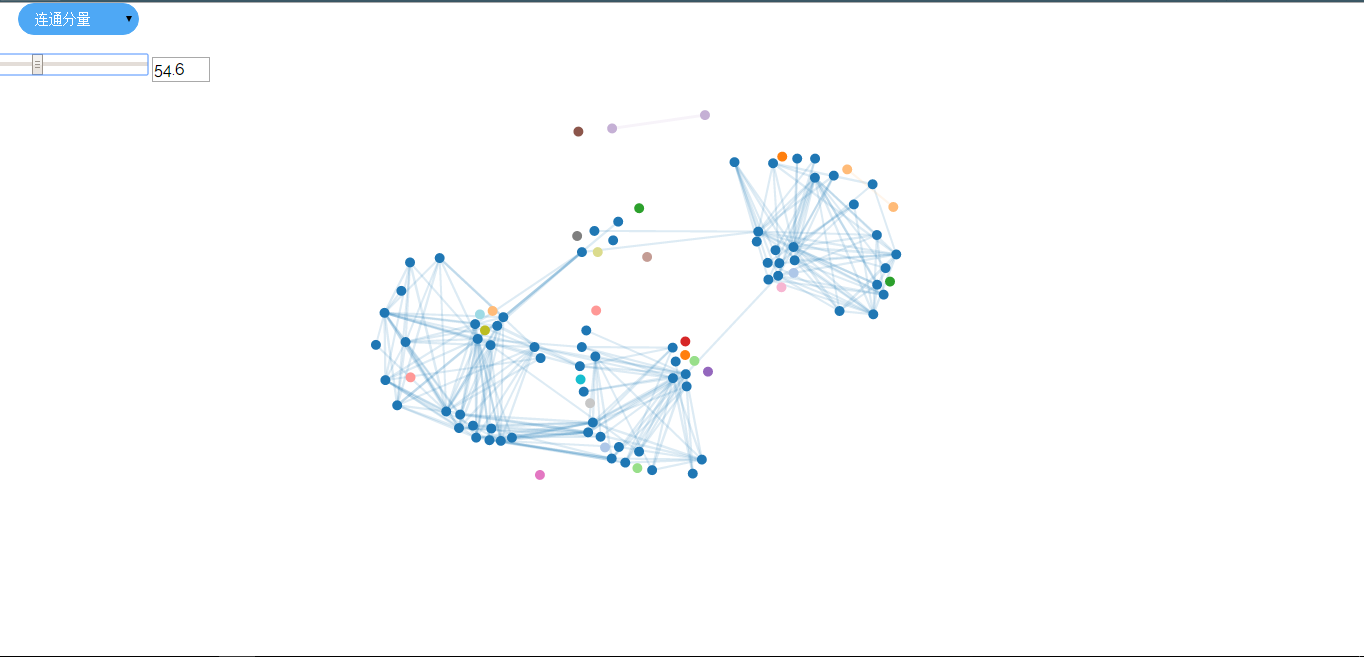
\includegraphics[width=0.9\linewidth]{connected_component.PNG}
		    \figcaption{连通分量—效果预览}
		\end{minipage} 
		\\[\intextsep] 		
		% subsubsection 算法说明 (end)
% section 核心算法的实现 (end)

\section{总结} % (fold)
	\paragraph{}
	感觉图论大作业虽然分值不高,但真的很有难度,也可以让自己学到很多东西。我们学会了使用python写爬虫获得数据,学会了使用d3展示图以及基本的交互,还学习了html的各种控件的使用,css的写法。同时用js实现相关算法,并且进行展示。感觉几天的刷夜,可以做出来一个如此漂亮的界面,非常开心,也有非常大的收获!
		
% section 总结 (end)

\end{CJK}
\end{document}
